\documentclass[tikz]{standalone}
\usepackage{pgfplots}
\pgfplotsset{compat=1.18}
\begin{document}
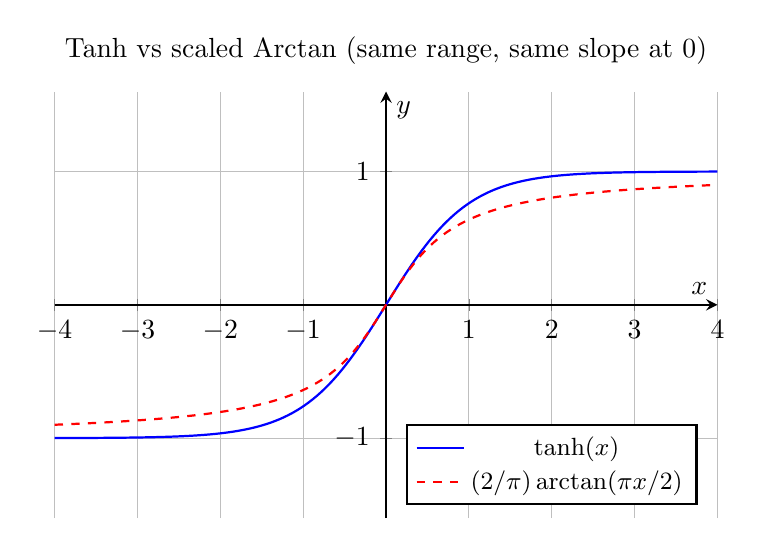
\begin{tikzpicture}
\begin{axis}[
  width=10cm, height=7cm,
  xlabel=$x$, ylabel=$y$,
  title={Tanh vs scaled Arctan (same range, same slope at 0)},
  xmin=-4, xmax=4, ymin=-1.6, ymax=1.6,
  axis x line=middle, axis y line=middle,
  grid=major, legend pos=south east,
  legend style={font=\small},
  samples=200, thick,
]
% tanh(x) = (e^{2x}-1)/(e^{2x}+1)
\addplot[blue] {(exp(2*x)-1)/(exp(2*x)+1)};
\addlegendentry{$\tanh(x)$}
% (2/pi)*atan(pi*x/2): atan() is in degrees, atan(u)/90 == (2/pi)*atan_rad(u)
\addplot[red, dashed] {atan(pi*x/2)/90};
\addlegendentry{$(2/\pi)\arctan(\pi x/2)$}
\end{axis}
\end{tikzpicture}
\end{document}
